\chapter{Language Implementation}


\section{Implementation process}

The implementation involves multiple steps: conceptual design of the DSL, creating the grammar, the lexer and parser, the testing functionality, and testing the DSL itself. Finally, it will be connected all together to work as a fully-fledged Domain Specific Language.

Conceptual design involves specifying the domain of the DSL, what problems it solves, defining use cases, how it will work, what it should and should not do.

Grammar is based on the syntax defined on the previous step. It involves knowing what types and functionality the language will contain.

There are different tools to implement a Domain Specific Language. ANTLR (ANother Tool for Language Recognition) is one of them. It gives a powerful parser that can be used for reading, processing, executing, or translating structured text or binary files. It works by defining a grammar. Then ANTLR creates a parser along with a parse tree. The parser can be used to parse code in the DSL and to apply different actions, which are written in the target language. The actions will do the unit testing behind the scenes for the scenarios specified for testing by the DSL.

There is another tool textX, inspired by a language workbench for building DSLs in java: Xtext. It is a meta-language for textual DSLs in Python. It is similar to ANTLR. Given a grammar description it builds a meta-model as Python classes and a parser for the language. The parser will automatically build a graph of Python objects corresponding to the meta-model. Other features include:
\begin{itemize}
    \item Automatic Abstract Syntax Tree construction
    \item Automatic linking, which allows to have references to other objects in the language and the textual representation of the reference will be resolved automatically
    \item Automatic parent-child relationships imposed by the grammar
    \item Parser configuration, to allow control of the whitespace characters, cases, keyword handling
    \item Model/object post-processing: validation, additional changes etc.
    \item Grammar modularization: grammar can be split across multiple files and imported when necessary
    \item Scope providers
    \item Multiple meta-models support
    \item Meta-model or model visualization with the GraphViz package
\end{itemize}

Xtext, that textX is based on, uses as a default a Concrete Syntax (CS) first approach. From a concrete syntax definition, an abstract syntax (AS) is derived. This is convenient. Though, the resulting AS may not be as clean as if it was derived manually.  The tool supports AS first approach too.

It was used a parser, this means that the abstract syntax tree (AST) is constructed from the CS of a program text. It instantiates and populates the AS, based on the information in the program.

\section{Working in ANTLR}
ANother Tool for Language Recognition (ANTLR) is a powerful tool for creating parsers, interpreters, compilers, and other language processing tools.

The grammar definition developed specifies the syntax for a testing domain-specific language (DSL). The grammar defines several rules that describe how the testing DSL should be structured.

\begin{verbatim}
grammar grammar_antlr;

suite: 'Suite' ID (test | order)*;
test: 'Test' ID flag* 'When' parameter+ result;
flag: '-' ('skip' | 'Skip' | 'Repeat' INT 'times');
parameter: ID '=' datatype | emptyParameters;
result: 'Then' ('result' 'should' 'be')? (datatype | emptyResult);
emptyParameters: 'no' 'parameters' | 'None' | 'none' | 'void' | 'Void';
emptyResult: 'empty' | 'Empty' | 'void' | 'Void' | 'none' | 'None';
order: 'Execution' 'order' ':' ID (',' ID)*;

datatype: STRING | INT | FLOAT | NUMBER | BOOL;
ID: [a-zA-Z_] [a-zA-Z0-9_]*;
STRING: '"' ~'"'* '"';
NUMBER: INT | FLOAT;
INT: [0-9]+;
FLOAT: [0-9]* '.' [0-9]+;
BOOL: 'true' | 'false';

WS: [ \t\r\n]+ -> skip;
\end{verbatim}

The first rule is "suite", which specifies that a suite consists of the word "Suite" followed by an identifier (ID) and zero or more tests or orders.

The second rule is "test", which specifies that a test consists of the word "Test" followed by an identifier, zero or more flags, the word "When", one or more parameters, and the word "Then" followed by an expected result.

The "flag" rule defines the optional flags that can be associated with a test, such as "skip" or "repeat".

The "parameter" rule defines the parameters that can be passed to a test.

The "result" rule defines the expected result of a test.

The "emptyParameters" and "emptyResult" rules define possible values for empty parameters and empty results, respectively.

The "order" rule specifies the execution order for the tests.

Finally, the "datatype" rule defines the possible data types for parameters and results, including strings, integers, floats, and booleans.

The grammar also defines the "WS" rule, which specifies that whitespace characters should be ignored.


\section{Converting tests into JSON}

Converting the tests generated from the grammar into JSON can provide compatibility with other programming languages and tools that can read and parse JSON. This allows the tests to be used in different contexts and environments, such as in continuous integration and deployment pipelines, where different programming languages and tools may be used.

JSON is a widely used data interchange format that is lightweight, easy to read and write, and can be easily consumed by a wide range of programming languages and tools. By converting the tests into JSON, they can be easily shared and used across different systems and platforms. Additionally, JSON is human-readable and can be easily understood by developers, which can make it easier to debug and troubleshoot issues in the tests.

In figure 4 there is a representation of a test implementation of the domain specific language for unit testing that was created.

{ \centering 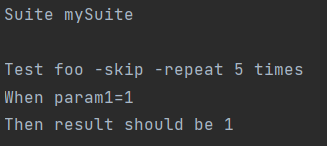
\includegraphics[width=\textwidth , height=6cm]{images/test1.png} }
\begin{center} Figure 4: Test example \end{center}

As noticed, in figure 5, the test was generated as a JSON in a external file.The advantage of converting the tests generated from the grammar into JSON is that it provides a standardized format that can be easily parsed and used to work with different programming languages.

{ \centering 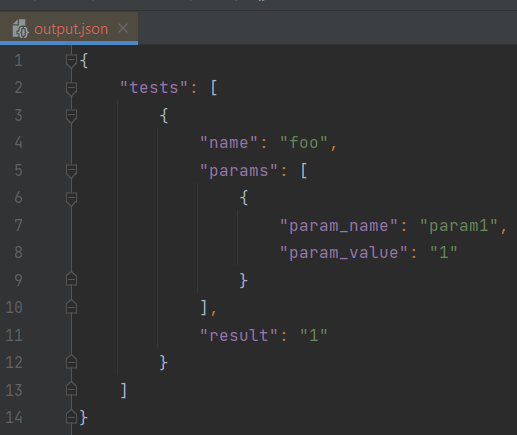
\includegraphics[width=\textwidth, height=12cm]{images/output.png} }
\begin{center} Figure 5: JSON output file  \end{center}

\section{Syntax Analyses}
In language processing, syntax analysis is an essential component of a parser. The process of examining the structure of a given sequence of tokens according to the rules of a formal grammar is known as syntax analysis, often known as parsing. It is a critical stage in the compilation or interpretation of computer languages.

A parser examines the stream of tokens created by the lexer (lexical analysis) to see if the token sequence follows the grammar rules of the language. It validates the syntax, determines the program's hierarchical structure, and generates a parse tree or an abstract syntax tree (AST) as a representation of the program's structure.

The input and output of a sample scenario requiring syntax analysis in the context of a testing suite are represented by the examples below. 

The input describes a set of tests organized within a suite. Each test has a name, potential parameters, an expected result, and optional flags such as "skip" and "repeat."

\begin{verbatim}
    Suite mySuite

    Test foo -skip -repeat 5 times
    When param1=1
    Then result should be 1

    Test foo2
    When param2=True, param3="John"
    Then result should be empty

    Test foo3 -skip
    When no parameters
    Then result should be 1.42

    Execution order: foo3, foo1, foo2
\end{verbatim}

The output is a structured representation of the input, indicating the suite name, the list of tests with their respective properties (name, parameters, result, skip status, and repetition count), and the execution order of the tests.

Considering that the DSL is specifically designed for unit testing purposes, it has been determined that representing the syntax analysis results as a dictionary is a more favorable approach, beacause Dictionaries allow easy access and modification of the parsed elements using key-value pairs and Flexibility: Dictionaries offer flexibility in terms of how the parsed structure is represented and organized.

\begin{verbatim}
{
    "suite": {
        "name": "mySuite",
        "tests": [
            {
                "name": "foo",
                "params": [
                    {
                        "name": "param1",
                        "type": "NUMBER",
                        "value": 1
                    }
                ],
                "result": 1,
                "skip": true,
                "num_repetitions": 5
            },
            {
                "name": "foo2",
                "params": [
                    {
                        "name": "param2",
                        "type": "BOOLEAN",        
                        "value": true
                    },
                    {
                        "name": "param3",
                        "type": "STRING",
                        "value": "John"
                    }
                ],
                "result": null,
                "skip": false,
                "num_repetitions": 1
            },
            {
                "name": "foo3",
                "params": [],
                "result": 1.42,
                "skip": true,
                "num_repetitions": 1
            }
        ],
        "executionOrder": [
            "foo3",
            "foo1",
            "foo2"
        ]
    }
}
\end{verbatim}

In this example, the syntax analysis is performed on the input to extract meaningful information and ensure it to the expected format.

During the syntax analysis, the input is processed to identify and validate different components, such as the suite name, test names, parameters, expected results, flags, and execution order. Syntax rules and patterns are used to determine the structure and relationships between these elements.



\section{Semantic Analyses}
The semantic analysis step of language processing comes after syntactic analysis. While syntax analysis focuses on the structure and arrangement of tokens according to grammar rules, semantic analysis investigates the program's meaning and accuracy.

The primary goal of semantic analysis is to detect and handle semantic flaws or inconsistencies that are not obvious from syntax alone. It entails inspecting the program's context and semantics to ensure that it follows the rules and limitations of the language.

Several operations are performed by the parser or a separate semantic analyzer during semantic analysis, including:

\begin{itemize}
    \item Type checking ensures consistency and correctness by verifying that expressions and statements are utilized with compatible types. It is verified, for instance, whether an arithmetic operation is done between compatible numeric types or whether a function is called with the correct number and kinds of arguments.
    \item It is monitoring the scope and visibility of variables, functions, and other program symbols. It ensures that symbols are defined before to use and that no name conflicts exist inside a particular scope.
    \item Symbol table generation involves creating a symbol table or symbol information repository that stores various symbols (such as variables, functions, classes, etc.) created in the program, along with their attributes and scope information. The symbol table proves useful in subsequent stages of compilation or interpretation.

    \item The input program is typically converted into an intermediate representation (IR), which serves as a lower-level representation that can be further processed or optimized. The generation of the symbol table aids in organizing and managing these symbols within the IR.
    \item Semantic error detection and reporting involves the identification and reporting of semantic issues in a program that cannot be discovered solely through syntax analysis. These issues include incompatible assignments, undeclared variables, or erroneous function calls.
\end{itemize}

The input could be modified and it is observed that if a string that is not a subset of the code is provided, it would output a message indicating the presence of an illegal token.

For instance, if is forgotten to write "parameters" in the When clause that expects no parameters like this:

\begin{verbatim}
        When no empty
\end{verbatim}

Then it should be output the following message:
 
\begin{verbatim}
        Syntax error! Expected 'no parameters' after `When`, got 'no empty'.
\end{verbatim}

The process of semantic analysis enhances the understanding of the program's intended meaning and identifies potential flaws that could result in run time errors or undesired behavior. By performing these tasks, semantic analysis helps ensure the correctness and reliability of the program by catching errors that may arise due to incorrect usage or inconsistencies in the program's semantics.

\section{Demonstration of the language}

The input demonstrates the usage of the language, featuring a suite named "mySuite" and several test cases. Each test case is identified by a name (e.g., "foo1", "foo2", "foo3") and is associated with potential parameters. The "When" clause defines the conditions for the test case, specifying the values of specific parameters (e.g., "param1=1", "param2=True", "param3='John'"). The "Then" clause expresses the expected result for each test case.

The input also provides an execution order, indicating the desired sequence in which the test cases should be executed. According to the given order, "foo3" is intended to be executed first, followed by "foo1", and finally "foo2".

\begin{verbatim}

       Suite mySuite

      Test foo1 -repeat 5 times
      When param1=1
      Then result should be 1

      Test foo2 -repeat 2 times
      When param2=True, param3="John"
      Then result should be 0

      Test foo3 
      When no parameters
      Then result should be 1.42

      Execution order: foo3, foo1, foo2
      
\end{verbatim}

Based on the data from Figure 6, it is clear that the tests were carried out successfully and without issue. The test execution order was strictly followed to, ensuring that the desired sequence was maintained throughout the testing procedure. Furthermore, the number of repetitions indicated for each test was taken into consideration effectively during execution, resulting in accurate and dependable test results. The fact that the tests passed implies that the language implementation and underlying testing framework worked as intended, indicating the efficacy of the testing techniques as well as the correctness of the execution order and repeat settings.

{ \centering 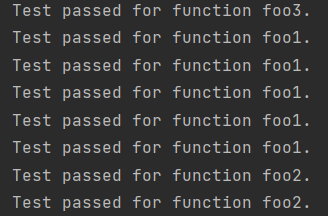
\includegraphics[width=\textwidth, height=10cm]{images/demo1.png} }
\begin{center} Figure 6: Output of the language \end{center}

Finally, the language demonstration highlighted the effective execution and passing of the tests. The adherence to the prescribed execution order and the appropriate management of test repetitions confirmed the language's and its related testing framework's dependability and accuracy. The demonstration highlighted the language's usefulness in facilitating unit testing and ensuring the desired outcomes by displaying the accurate execution and expected results of the tests.
